\documentclass[10pt,twocolumn,letterpaper]{article}

\usepackage{cvpr}
\usepackage{times}
\usepackage{epsfig}
\usepackage{graphicx}
\usepackage{amsmath}
\usepackage{amssymb}
\usepackage{subfigure}
\usepackage{upgreek}

% Include other packages here, before hyperref.

% If you comment hyperref and then uncomment it, you should delete
% egpaper.aux before re-running latex.  (Or just hit 'q' on the first latex
% run, let it finish, and you should be clear).
\usepackage[pagebackref=true,breaklinks=true,letterpaper=true,colorlinks,bookmarks=false]{hyperref}

% \cvprfinalcopy % *** Uncomment this line for the final submission

\def\cvprPaperID{****} % *** Enter the CVPR Paper ID here
\def\httilde{\mbox{\tt\raisebox{-.5ex}{\symbol{126}}}}

% Pages are numbered in submission mode, and unnumbered in camera-ready
\ifcvprfinal\pagestyle{empty}\fi
\begin{document}

%%%%%%%%% TITLE
\title{External Patch Group Prior Guided Internal Subspace Learning for Real Image Denoising}

\author{First Author\\
Institution1\\
Institution1 address\\
{\tt\small firstauthor@i1.org}
% For a paper whose authors are all at the same institution,
% omit the following lines up until the closing ``}''.
% Additional authors and addresses can be added with ``\and'',
% just like the second author.
% To save space, use either the email address or home page, not both
\and
Second Author\\
Institution2\\
First line of institution2 address\\
{\tt\small secondauthor@i2.org}
}

\maketitle

%%%%%%%%% ABSTRACT
\begin{abstract}
Existing image denoising methods largely depends on noise modeling and estimation. The commonly used noise models, additive white Gaussian, are inflexible in describing the complex noise on real noisy images. This would limit the performance of existing methods on denoising real noisy images. In this paper, we firstly demonstrate that almost all state-of-the-art methods on removing Gaussian noise and real noise are limited in denoising real noisy images. We demonstrate that a simple Patch Group based Prior Learning model on RGB images can achieve better performance than existing denoising methods, especially the ones designed for real noise in natural images. Besides, we employ the external patch group prior learning for internal clustering and subspace learning. This external inormation guided internal denoising methods acheives even better than the external PG prior based methods and the fully internal PG prior based method. Through extensive on standard datasets on real noisy images with groundtruth, we demonstrate that the proposed method achieves much better denoising performance than the other state-of-the-art methods on Gaussian noise removal and real noise removal. 
\end{abstract}

%%%%%%%%% BODY TEXT
\section{Introduction}
Image denoising is a fundermental problem in computer vision and image processing. It is an ideal platform for testing natural image models and provides high-quality images for other conputer vision tasks such as image registration, segmentation, and pattern recognition, etc. For several decades, there emerge numerous image denoising methods \cite{nlm,foe,ksvd,bm3d,lssc,epll,mlp,wnnm,csf,pgpd,chen2015learning}, and all of them focus mainly on dealing with additive white Gaussian noise (AWGN). However, the images captured by CMOS or CCD cameras will undertake an in-camera imaging pipeline. The in-camera imaging pipeline includes mainly image demosaicing, white balance and color space transform, gamut mapping, tone mapping, and JPEG comression \cite{NewInCamera,crosschannel2016}. Therefore, the noise in real images are much more complex than Gaussian, and depends on camera series, brands, as well as the settings (ISO, shutter speed, and aperture, etc). The models designed to deal with AWGN would become much less effective on real noisy images.

%Recently, several discriminative learning methods \cite{burger2012image,csf,chen2015learning} achieving expressive performance on Gaussian noise removal. These methods require a set of paired images, namely clean ground-truth images and the simulated noisy counterparts degraded by identical noise (mainly additive white Gaussian noise, AWGN), to learn an effective model for image denoising. 

In the last decade, the methods of \cite{fullyblind,rabie2005robust,Liu2008,almapg,noiseclinic,Zhu_2016_CVPR,crosschannel2016} are designed to deal with real noisy images. Almost all these methods coincidently employ a two-stage framework: in the first stage, assuming a distribution model (usually Gaussian) on the noise and estimate its parameters; in the second stage, performing denoising with the help of the noise modeling and estimation in the first stage. However, the Gaussian assumption is inflexible in describing the complex noise on real noisy images \cite{Liu2008}. Although the mixture of Gaussians (MoG) model is possible to approximate any unknown noise \cite{Zhu_2016_CVPR}, estimating its parameters is often time consuming via nonparametric Bayesian techniques \cite{Zhu_2016_CVPR,Bishop}. To evaluate the performanec of these methods on dealing with complex real noise, we apply these methods, with corresponding default parameters, on a real noisy image provided in \cite{crosschannel2016}. This image is captured by a Nikon D800 camera while the ISO is set as 3200. The "ground truth" image is also provided with which we can calculate objective measurements. More details about this dataset can be found at the experimental section. The denoised images are listed in Figure \ref{fig1}, from which we can see that these methods either remove the noise or oversmooth the complex details in real noisy image. This proves that the above mentioned methods are not effective on denoising complex noise on real images. 
\begin{figure*}\label{fig1}
\centering
\subfigure{
\begin{minipage}[t]{0.2\textwidth}
\centering
\raisebox{-0.15cm}{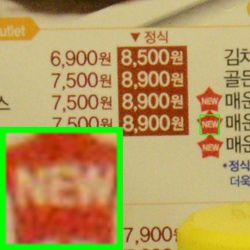
\includegraphics[width=1\textwidth]{images/resize_br_Noisy_CC_Noisy_Nikon_D800_ISO_3200_A3_66.png}}
{\footnotesize (a) Noisy Image \\ (33.30dB/0.8921) }
\end{minipage}
\begin{minipage}[t]{0.2\textwidth}
\centering
\raisebox{-0.15cm}{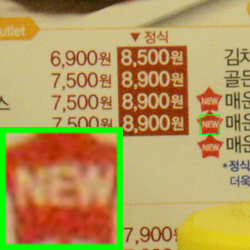
\includegraphics[width=1\textwidth]{images/resize_br_CBM3D_CC_Noisy_Nikon_D800_ISO_3200_A3_66.png}}
{\footnotesize (b) CBM3D \cite{cbm3d} \\ (33.33dB/0.8935)  }
\end{minipage}
\begin{minipage}[t]{0.2\textwidth}
\centering
\raisebox{-0.15cm}{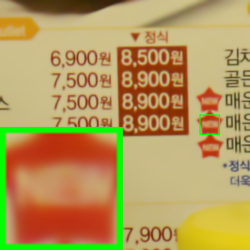
\includegraphics[width=1\textwidth]{images/resize_br_MLP_CC_Noisy_Nikon_D800_ISO_3200_A3_66.png}}
{\footnotesize (c) MLP \cite{mlp}\\ (34.22dB/0.9603) }
\end{minipage}
\begin{minipage}[t]{0.2\textwidth}
\centering
\raisebox{-0.15cm}{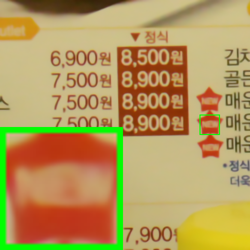
\includegraphics[width=1\textwidth]{images/resize_br_CSF_CC_Noisy_Nikon_D800_ISO_3200_A3_66.png}}
{\footnotesize (d) CSF \cite{csf}\\ (35.39dB/0.9677) }
\end{minipage}
\begin{minipage}[t]{0.2\textwidth}
\centering
\raisebox{-0.15cm}{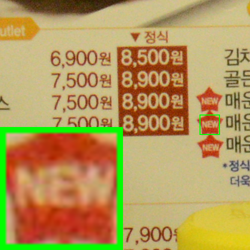
\includegraphics[width=1\textwidth]{images/resize_br_WNNM_CC_Noisy_Nikon_D800_ISO_3200_A3_66.png}}
{\footnotesize (e) WNNM \cite{wnnm}\\ (33.30dB/0.8922)  }
\end{minipage}
}
\subfigure{
\begin{minipage}[t]{0.2\textwidth}
\centering
\raisebox{-0.15cm}{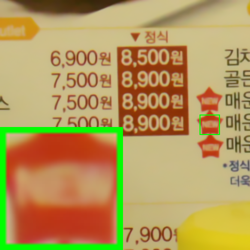
\includegraphics[width=1\textwidth]{images/resize_br_TRD_CC_Noisy_Nikon_D800_ISO_3200_A3_66.png}}
{\footnotesize (f) TRD \cite{chen2015learning} \\ (35.97dB/0.9705)   }
\end{minipage}
\begin{minipage}[t]{0.2\textwidth}
\centering
\raisebox{-0.15cm}{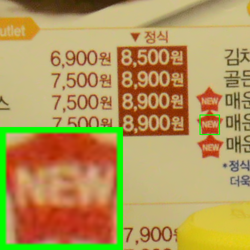
\includegraphics[width=1\textwidth]{images/resize_br_NC_CC_Noisy_Nikon_D800_ISO_3200_A3_66.png}}
{\footnotesize (g) PGPD \cite{pgpd} \\ (35.33dB/0.9520)  }
\end{minipage}
\begin{minipage}[t]{0.2\textwidth}
\centering
\raisebox{-0.15cm}{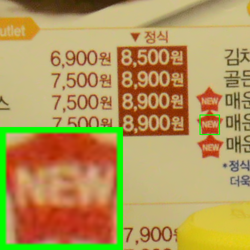
\includegraphics[width=1\textwidth]{images/resize_br_NC_CC_Noisy_Nikon_D800_ISO_3200_A3_66.png}}
{\footnotesize (h) Noise Clinic \cite{noiseclinic} \\ (35.33dB/0.9520)  }
\end{minipage}
\begin{minipage}[t]{0.2\textwidth}
\centering
\raisebox{-0.15cm}{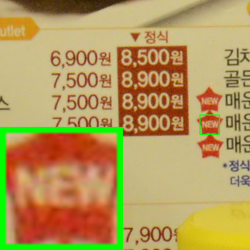
\includegraphics[width=1\textwidth]{images/resize_br_NI_CC_Noisy_Nikon_D800_ISO_3200_A3_66.png}}
{\footnotesize (i) Neat Image \cite{neatimage}\\ (34.39dB/0.9314)  }
\end{minipage}
\begin{minipage}[t]{0.2\textwidth}
\centering
\raisebox{-0.15cm}{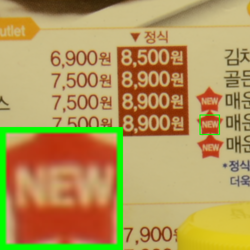
\includegraphics[width=1\textwidth]{images/resize_br_Mean_CC_Noisy_Nikon_D800_ISO_3200_A3_66.png}}
{\footnotesize (j) Mean Image }
\end{minipage}
}
\caption{Denoised images of the real noisy image "$Nikon D800 ISO 3200 A3$" by different methods. The images are better to be zoomed in on screen.}
\end{figure*}

In this paper, we attempt to deal with complex noise in real images by intergrating the external and internal information. Since the real noise is signal dependent \cite{crosschannel2016,healey1994radiometric}, the prior information in external natural images can be employed to avoid the high correlation between noise and siganl in internal images. On the other hand, the internal prior is adaptive to the image and can recover better the latent clean image. Based on these observations, we make detailed study on internal and external information for real image denoising task. We made several observations. Firstly, we found that the Patch Group Prior learning based denoising method \cite{pgpd} learned on clean RGB images are enough to outperform the above mentioned denoising methods. Secondly, we also found that a fully internal PG prior based denoising method which achieve better performance than the fully external method. Most importantly, we found that the external PG prior guided internal method can achieve even better and faster performance on real image denoising. In fact, the external PG prior learning based model is employed to guide the clustering of internal PGs extracted from the input noisy images. Then for each cluster of PGs, we perform subspace learning by PCA and denoising by weighted sparse coding. We perform comprehensive experiments on real noisy images captured by different CMOS or CCS sensors. The results demonstrate that our method achieves comparable or even better performance on denoising real noisy images. This reveals the potential advantages of combining external and internal information o natural images on robust and complex real noisy image denoising problem.

\subsection{Our Contributions}
The contributions of this paper are summarized as follows:
\begin{itemize}
\item We propose a noval method which combine the external and internal PG prior for real noisy image denoising problem;
\item Our method doesn't need noise modeling and estimation, and the noise levels of real noisy images are automatically expresssed by the singular values of learned subspace;
\item We achieve much better performance on visual quality, PSNR, SSIM, and speed, than other competing methods for real image denoising problem.
\end{itemize}

The rest of this paper will be summerized as follows: in Section 2, we will introduce the related work close to our work; in Section 3, we will introduce our proposed external prior guided internal subspace learning framework for real image denoising; in Section 4, we will demonstrate the denoising experiments on several standard dataset; in Section 5, we will conclude our paper and give our future work.
\section{Related Work}
\subsection{Patch Group Prior of Natural Images}
Patch prior is an approximation of the prior of natural images. There are several famous work on this area such as the K-SVD algorithm \cite{ksvd}. The seminar work on patch prior modeling is the expected patch log likelihood (EPLL), which models the space of natural image patches via Gaussian Mixture Model. Recently, the Patch Group prior \cite{pgpd} is proposed to directly model the non-local self similarity within natural images. The patch group prior demonstrate better properties via better image denoising performance on natural images. However, PGPD only utilizes the information of clean natural images, but not fully make full of the NSS information of noisy input images. In this paper, we combine the information of external natural clean images and internal real noisy images to achieve adaptive patch group prior modeling. In fact, we use the external Pacth Group prior to guide the structural clustering of internal patch groups in real noisy images. For each cluster of PGs, we propose to use PCA for subspace learning. The eigenvectors are the basis of this subspace and hence can be used as an orthonormal dictionary. The eigenvalues reflect the information describing the noise levels and hence can be used as parameters for image denoising. Noted that the dictionary and parameters are obtained via a fully unsupervised way by subspace learning. Therefore, our model is highly adaptive to the noisy input images.


\subsection{Internal v.s. External Image Denoising}
The internal patch recurrence across multiple scales of a natural image has been successfully applied in many image restoration problems such as single image super-resolution \cite{Irani2009sr}, image denoising \cite{Irani2013separating}, blind image deblurring \cite{Irani2014deblur}, and image dehazing \cite{Irani2016dehazing}, etc. These work demonstrate that internal information is enough for denoising additive white Gaussian noise. The reason is that the AWGN noise is independent of the original clean images, and therefore it will be 缩小 when the image is scaled to smaller size. However, the real noise is dependent on the signal \cite{crosschannel2016} and it has fixed patterns from several main sources \cite{healey1994radiometric}. The internal information may be not enough for real image denoising problem. Noted that even in denoising AWGN, the introduce of external information will also improve the performance denoising methods \cite{luo2015adaptive}. In this paper, we demonstrate that for real noise which is signal dependent, it is essential to make use of external clean data.

\subsection{Real Image Denoising}
To the best of our knowledge, the study of real image denoising can be dated back to the BLS-GSM model \cite{blsgsm}, in which Portilla et al. proposed to use scale mixture of Gaussian in overcomplete oriented pyramids to estimate the latent clean images. In \cite{fullyblind}, Portilla proposed to use a correlated Gaussian model for noise estimation of each wavelet subband. Based on the robust statistics theory \cite{huber2011robust}, the work of Rabie \cite{rabie2005robust} modeled the noisy pixels as outliers, which could be removed via Lorentzian robust estimator. In \cite{Liu2008}, Liu et al. proposed to use 'noise level function' (NLF) to estimate the noise and then use Gaussian conditional random field to obtain the latent clean image. Recently, Gong et al. proposed an optimization based method \cite{almapg}, which models the data fitting term by weighted sum of $\ell_{1}$ and $\ell_{2}$ norms and the regularization term by sparsity prior in the wavelet transform domain. Later, Lebrun el al. proposed a multiscale denoising algorithm called 'Noise Clinic' \cite{noiseclinic} for real image denoising task. This method generalizes the NL-Bayes \cite{nlbayes} to deal with signal, scale, and frequency dependent noise. Recently, Zhu et al. proposed a Bayesian model \cite{Zhu_2016_CVPR} which approximates the noise via Mixture of Gaussian (MoG) model \cite{Bishop}. The clean image is recovered from the noisy image by the proposed Low Rank MoG filter (LR-MoG). However, noise level estimation is already a challenging problem and denoising methods are quite sensitive to this parameter. Moreover, these methods are based on shrinkage models that are too simple to reflect reality, which results in over-smoothing of important structures such as small-scale text and textures. 

\section{External Patch Group Prior Guided Internal Subspace Learning}
In this section, we formulate the framework of external Patch Group prior guided internal subspace learning. We first introduce the patch group prior leaning on clean natural RGB images. Then we formulate the external guided internal subspace learning. Finally, we discuss the differences between external subspaces and the corresponding internal subspace.

\subsection{External Patch Group Prior Learning on Clean Natural Images}
Images often demonstrate highly nonlocal self-similarity (NSS) property, which refers to the fact that a patch always have similar patches to it around the image. This property is a key successful factor in image denoising methods \cite{nlm,bm3d,lssc,ncsr,wnnm} and restoration methods \cite{}. In \cite{pgpd}, the NSS property is recently learned as an external prior in a patch group manner. In this section, we formulate the Patch Group prior on clean natural images.

In external PG prior learning on clean natural images, a PG is obtained via finding the $M$ most similar nonlocal patches to the local patch (size: $p\times p \times 3$ for RGB channels) in a given clean image. The similarity is measured by Euclidean distance or other distance measurements. In this work, we find similar PGs through the Euclidean distance based block matching in a large enough local window of size $W\times W$. The PG is denoted by $\{\mathbf{x}_{m}\}_{m=1}^{M}$, where $\mathbf{x}_{m}\in \mathbb{R}^{3p^{2}\times1}$ is a patch vector. The mean vector of this PG is $\boldsymbol{\upmu}=\frac{1}{M}\sum_{m=1}^{M}\mathbf{x}_{m}$, and $\mathbf{\overline{x}}_{m}=\mathbf{x}_{m}-\boldsymbol{\upmu}$ is the group mean subtracted patch vector. We call
\begin{equation}\label{equ1}
\mathbf{\overline{X}}\triangleq \{\mathbf{\overline{x}}_{m}\}, m=1,...,M
\end{equation}
the group mean subtracted PG, and it will be used to learn the NSS prior in our work. All these are similar with the definitions in \cite{pgpd}. 

From a given set of natural images, we can extract $N$ PGs, and  PG as
\begin{equation}\label{equ2}
\mathbf{\overline{X}}_{n}\triangleq \{\mathbf{\overline{x}}_{n,m}\}_{m=1}^{M}, n=1,...,N.
\end{equation}
We employ the patch group based Gaussian Mixture Model (PG-GMM) for NSS prior learning. The learning process is the same with that in \cite{pgpd}.

With PG-GMM, we aim to learn a set of $K$ Gaussians $\{\mathcal{N}(\boldsymbol{\upmu}_{k},\mathbf{\Sigma}_{k})\}$ from $N$ training PGs $\{\mathbf{\overline{X}}_{n}\}$, while requiring that all the $M$ patches $\{\mathbf{\overline{x}}_{n,m}\}$  in PG $\mathbf{\overline{X}}_{n}$ belong to the same Gaussian component and assume that the patches in the PG are independently sampled. Note that such an assumption is commonly used in patch based image modeling \cite{ksvd,lssc}. Then, the likelihood of $\{\mathbf{\overline{X}}_{n}\}$ can be calculated as
\begin{equation}\label{equ3}
P(\mathbf{\overline{X}}_{n})  = \sum\nolimits_{k=1}^{K}\pi_{k}\prod\nolimits_{m=1}^{M}\mathcal{N}(\mathbf{\overline{x}}_{n,m}|\boldsymbol{\upmu}_{k},\mathbf{\Sigma}_{k}).
\end{equation}
By assuming that all the PGs are independently sampled, the overall objective log-likelihood function is
\begin{equation}\label{equ4}
\begin{split}
\ln\mathcal{L}=\sum_{n=1}^{N} \ln(\sum_{k=1}^{K}\pi_{k}\prod_{m=1}^{M}\mathcal{N}(\mathbf{\overline{x}}_{n,m}|\boldsymbol{\upmu}_{k},\mathbf{\Sigma}_{k})).
\end{split}
\end{equation} 
We maximize the above objective function for PG-GMM learning. Finally, we obtain the GMM model with three sets of parameters including mixture weights $\{\pi_{k}\}_{k=1}^{K}$, mean vectors $\{\boldsymbol{\upmu}_{k}=\mathbf{0}\}_{k=1}^{K}$, and covariance matrices $\{\mathbf{\Sigma}_{k}\}_{k=1}^{K}$. Noted that in PGPD \cite{pgpd}, the mean vector of each cluster is natural zeros, i.e., $\boldsymbol{\upmu}_{k}=\mathbf{0}$.

\subsection{External PG Prior Guided Internal Subspace Learning}
For each $\mathbf{\overline{Y}}$, we select the most suitable Gaussian component to it from the trained PG-GMM. Since the noise on real images are small when compared to the signals and the noise on real images are dependent on the signals, the covariance matrix of the $k$th component is still $\mathbf{\Sigma}_{k}$. The selection can be done by checking the posterior probability that $\mathbf{\overline{Y}}$ belongs to the $k$th Gaussian component:
\begin{equation}\label{equ8}
P(k|\mathbf{\overline{Y}})=\frac{\prod_{m=1}^{M}\mathcal{N}(\mathbf{\overline{y}}_{m}|\mathbf{0},\mathbf{\Sigma}_{k})}{\sum_{l=1}^{K}\prod_{m=1}^{M}\mathcal{N}(\mathbf{\overline{y}}_{m}|\mathbf{0},\mathbf{\Sigma}_{l})}.
\end{equation}
Finally, the component with the highest probability $\ln P(k|\mathbf{\overline{Y}})$ is selected to process $\mathbf{\overline{Y}}$.

Suppose that the $k$th Gaussian component is selected for PG $\mathbf{\overline{Y}}$. For notation simplicity, we remove the subscript $k$ and denote by $\mathbf{\Sigma}$ the covariance matrix of this component. In PG-GMM, the PGs actually represent the variations of the similar patches in a group, and these variations are assigned to the same Gaussian distribution. By singular value decomposition (SVD), $\mathbf{\Sigma}$ can be factorized as
\begin{equation}\label{equ10}
\mathbf{\Sigma} = \mathbf{D}\mathbf{\Lambda}\mathbf{D}^{T},
\end{equation}
where $\mathbf{D}$ is an orthonormal matrix composed by the eigenvectors of $\mathbf{\Sigma}$ and $\mathbf{\Lambda}$ is the diagonal matrix of eigenvalues. With PG-GMM, the eigenvectors  in $\mathbf{D}$ capture the statistical structures of NSS variations in natural images, while the eigenvalues in $\mathbf{\Lambda}$ represent the significance of these eigenvectors. Fig.\ 4 shows the eigenvectors for 3 Gaussian components. It can be seen that these eigenvectors encode the possible variations of the PGs. For one Gaussian component, the first eigenvector represents its largest variation, while the last eigenvector represents its smallest variation. For different Gaussian components, we can see that their eigenvectors (with the same index) are very different. Hence, $\mathbf{D}$ can be used to represent the structural variations of the PGs in that component.

\begin{equation}\label{equ15}
\min\nolimits_{\boldsymbol{\upalpha}}\|\mathbf{\overline{y}}_{m}-\mathbf{D}\boldsymbol{\upalpha}\|_{2}^{2}+\sum_{i=1}^{p^{2}}\frac{c}{\mathbf{\lambda}_{i}}|\boldsymbol{\upalpha}_{i}|.
\end{equation}
By comparing (\ref{equ15}) with (\ref{equ11}), we can see that the $i$th entry of the weighting vector $\mathbf{w}$ should be
\begin{equation}\label{equ16}
\setlength{\abovedisplayskip}{3pt}
\setlength{\belowdisplayskip}{3pt}
\mathbf{w}_{i} = c/(\mathbf{\lambda}_{i}+\varepsilon),
\end{equation}
where $\varepsilon$ is a small positive number to avoid dividing by zero. With $\mathbf{w}$ determined by (\ref{equ16}), let's see what the solution of (\ref{equ11}) should be. Since the dictionary $\mathbf{D}$ is orthonormal, it is not difficult to find out that (\ref{equ11}) has a closed-form solution (detailed derivation can be found in the supplementary material):
\begin{equation}\label{equ17}
\setlength{\abovedisplayskip}{3pt}
\setlength{\belowdisplayskip}{4pt}
\hat{\boldsymbol{\upalpha}}= \text{sgn}(\mathbf{D^{T}\overline{y}}_{m})\odot \text{max}(|\mathbf{D^{T}\overline{y}}_{m}|-\mathbf{w}/2,0),
\end{equation}
where $\text{sgn}(\bullet)$ is the sign function, $\odot$ means element-wise multiplication, and $|\mathbf{D^{T}\overline{y}}_{m}|$ is the absolute value of each entry of vector $|\mathbf{D^{T}\overline{y}}_{m}|$. The closed-form solution makes our weighted sparse coding process very efficient. 
\vspace{-0.05in}

\subsection{What does External Data help the Internal Subspace Learning?}
The external data can help the internal learning in two ways. On one hand, it can guide the noisy image patches to be divided into correct subspaces through clustering. If we cluster the noisy patches in an automatical way, just like the PLE \cite{ple} did, the signal dependent noise would be hardly removed. With the help of clean external data, the noisy patches can be divided into correct subspaces. Besides, external data guided internal clustering is much more efficient than directly clustering the noisy data due to the time consuming fitting procedure. On the other hand, due to the correct division of internal noisy data, the dictionary and paranters for subspace learning could be more adaptive to the testing real noisy image. Hence, it would achieve better denoising performance than the methods only using the external information.

\subsection{The Internal PGs Spaces Are Subspaces of Corresponding External PG Spaces}
In this subsection, we compare the distribution of external PGs extracted from clean natural images and real noisy images. For better illumination, we randomly selected a cluster and project the original clean PGs onto a 2-D plane. Plot a Figure to demonstrate the data distributed in external space and the assigned internal subspace. The internal subspace is only a subspace of the external space. Hence, if we use the external data to perform denoising, the performance would be limited due to the dependence of noise on signal. If we combine the external and internal data for subspace learning, the learned subspace would be too generative and would therefore not specifically suitable for the testing data. 

\section{The Enhanced Algorithm}

\subsection{Iterative Regularization}
Perfoming image denoising in one iteration is not enough for real noise since the noise is signal dependent. The removed noise in one iteration is largely dependent on the signal. Therefore, it is essential to add back some residuals removed in this iteration for the denoising of the next iteration. 

\subsection{Effectively dealing with different noisy images}
For real image denoising, we can perform well on images which have similar noise levels with the training dataset. How can we deal with the real noisy images whose noise levels are higher than the training dataset? The answer is to remove the noise by more iterations. The input image of each iteration is the recovered image of previous iteration. This makes sense since we can still view the recovered image as a real noisy image. 

This will also bring a second problem, that how we could automatically terminate the iteration. This can be solved by two methods. One way is to compare the images between two iterations and calculate their difference, the iteration can be terminated if the difference is smaller than a threshold. The other way is to estimate the noise level of the current image and terminate the iterations when the noise level is lower than a preset threshold. We employ the second way and set the threshold as 0.0001 in our experiments. In fact, most of our testing images will be denoised well in one iteration.

\subsection{Efficient Model Selection by Gating Network}
In the Gaussian component selection procedure, if we employ the full posterior estimation, the speed is not fast. Our algorithm can be speeded up by introducing the Gating network model.

\subsection{The Overall Algorithm}



%------------------------------------------------------------------------
\section{Experiments}
In this section, we perform real image image denoising experiments on three standard datasets. The first dataset is real noisy images with mean images as ground truths provided by \cite{crosschannel2016}. The second dataset is provided by the website of Noise Clinic \cite{noiseclinic}. The third dataset is provided by the Commercial software Neat Image \cite{neatimage}. The second and third dataset do not have ground truth images.

\subsection{Parameters Setting}
The proposed method contains the PG prior learning stage, the external prior guided internal subspace learning stage, and the denoising stage. In the learning stage, similar to the PGPD, there are four parameters, $p$, $M$, $W$, and $K$.  We set $p=6$ and hence the patch size is $6\times 6 \times 3$. The winodw size for searching PGs is $W = 31$. The number of similar patches is $N=10$, the number of cluters is set as $K = 33$. In the external prior guided learning stage, there is no parameters. In the denoising stage, there are one paramters, i.e., the $\lambda$ which is used to regularize the sparse term.


\subsection{Comparison on External and Internal methods}
In this subsection, we compared the proposed external prior guided internal subspace learning model on real image denoising. The three methods are evaluated on the dataset provided in \cite{crosschannel2016}. We calculate the PSNR, SSIM \cite{ssim} and visual quality of these three methods. We also compare the speed. The PSNR and SSIM results on 60 cropped images from \cite{crosschannel2016} are listed in Table 1. The images are cropped into size of $500\times 500$ for better illustration. We also compare the three methods on visual quality in Figure \ref{fig2}.

\begin{figure*}\label{fig2}
\centering
\subfigure{
\begin{minipage}[t]{0.2\textwidth}
\centering
\raisebox{-0.15cm}{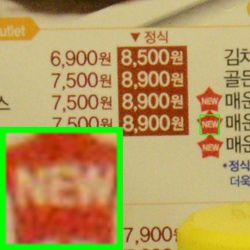
\includegraphics[width=1\textwidth]{images/resize_br_Noisy_CC_Noisy_Nikon_D800_ISO_3200_A3_66.png}}
{\footnotesize (a) Noisy Image \\ (33.30dB/0.8921) }
\end{minipage}
\begin{minipage}[t]{0.2\textwidth}
\centering
\raisebox{-0.15cm}{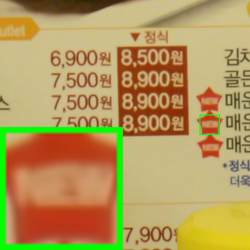
\includegraphics[width=1\textwidth]{images/resize_br_Offline_CC_Noisy_Nikon_D800_ISO_3200_A3_66.png}}
{\footnotesize (h) Offline \\ (36.29dB/0.9705)}
\end{minipage}
\begin{minipage}[t]{0.2\textwidth}
\centering
\raisebox{-0.15cm}{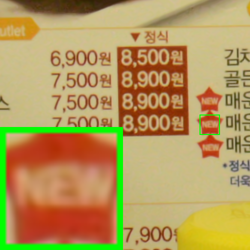
\includegraphics[width=1\textwidth]{images/resize_br_Online_CC_Noisy_Nikon_D800_ISO_3200_A3_66.png}}
{\footnotesize (i) Online \\ (35.80dB/0.9641) }
\end{minipage}
\begin{minipage}[t]{0.2\textwidth}
\centering
\raisebox{-0.15cm}{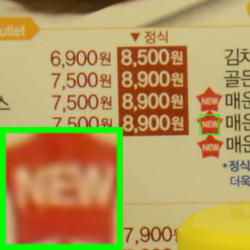
\includegraphics[width=1\textwidth]{images/resize_br_Guided_CC_Noisy_Nikon_D800_ISO_3200_A3_66.png}}
{\footnotesize (j) Guided \\ (\textbf{37.28}dB/\textbf{0.9729})}
\end{minipage}
\begin{minipage}[t]{0.2\textwidth}
\centering
\raisebox{-0.15cm}{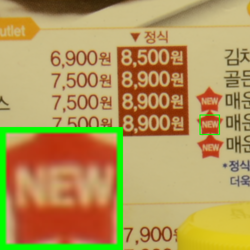
\includegraphics[width=1\textwidth]{images/resize_br_Mean_CC_Noisy_Nikon_D800_ISO_3200_A3_66.png}}
{\footnotesize (h) Mean Image }
\end{minipage}
}
\caption{Denoised images of the old image "$Nikon D800 ISO 3200 A3$" by different methods. The images are better to be zoomed in on screen.}
\end{figure*}


\subsection{Comparison With other Competing Methods}
We compare with previous state-of-the-art Gaussian noise removal methods such as BM3D \cite{bm3d}, WNNM \cite{wnnm}, MLP \cite{mlp}, CSF \cite{csf}, and the recently proposed TRD \cite{chencvpr2015}. We also compare with three competing real image denoising methods such as Noise Clinic, Neat Image, and the CCNoise method proposed recently. The popular software NeatImage which is one of the best denoising software available. All these methods need noise estimation which is vary hard to perform if there is no uniform regions are available in the testing image. The NeatImage will fail to perform automatical parameters settings if there is no uniform regions. \footnote{To compare with CCNoise, we first transform the denoised images into double format.}


\subsection{Real Image Denoising}

We  the competing denoising methods from various research directions on two datasets. Both the two datasets comes from the \cite{crosschannel2016}. The first dataset contains 17 images of size over $7000\times5000$. Since this dataset contains recurrent contents across different images, we crop 60 small images of size $500\times500$ from these 17 images in \cite{crosschannel2016}.

The PSNR and SSIM resluts are listed in table \ref{tab1}.
\begin{table*}\label{tab1}
\caption{Average PSNR(dB) results of different methods on 60 cropped real noisy images captured in \cite{crosschannel2016}.}
\label{tab1}
\begin{center}
\renewcommand\arraystretch{1}
\begin{tabular}{|c||c|c|c|c|c|c|c|c|c|c|c|c|}
\hline
Image & \textbf{Noisy} &\textbf{CBM3D}&\textbf{WNNM}&\textbf{MLP}&\textbf{CSF}&\textbf{TRD}& \textbf{NI}& \textbf{NC}&\textbf{Offline} &\textbf{Online} &\textbf{Guided} 
\\
\hline
PSNR & 34.51  &  34.58 &  34.52  & 36.19   & 37.40 & 37.75 &  36.53  &  37.57  &  38.19   & 38.07 &  \textbf{ 38.46}
\\
\hline
SSIM & 0.8718  & 0.8748  & 0.8743   & 0.9470 & 0.9598 &  0.9617 & 0.9241  &  0.9514  &  0.9663   & 0.9625 &   \textbf{0.9677}
\\
\hline
\end{tabular}
\end{center}
\end{table*}

\begin{table*}\label{tab2}
\caption{Average PSNR(dB) results of different methods on 15 cropped real noisy images used in \cite{crosschannel2016}.}
\label{tab1}
\begin{center}
\renewcommand\arraystretch{1}
\begin{tabular}{|c||c|c|c|c|c|c|c|c|c|c|c|c|}
\hline
Image & \textbf{Noisy} &\textbf{CBM3D}&\textbf{WNNM}&\textbf{MLP}&\textbf{CSF}&\textbf{TRD}& \textbf{NI}& \textbf{NC}& \textbf{CC}&\textbf{Offline} &\textbf{Online} &\textbf{Guided} 
\\
\hline
PSNR & 33.41  &  33.48 &  33.48  & 34.32   & 35.33 &  35.65 &  35.49   &  36.43  &  36.88  & 36.69 & 36.73 &  \textbf{ 37.04}
\\
\hline
SSIM & 0.8483  & 0.8511  & 0.8512   & 0.9113 & 0.9250 &  0.9280  & 0.9126  &  0.9364  & 0.9481  & 0.9479 & 0.9419 &  \textbf{ 0.9509}
\\
\hline
\end{tabular}
\end{center}
\end{table*}

\begin{figure*}
\centering
\subfigure{
\begin{minipage}[t]{0.2\textwidth}
\centering
\raisebox{-0.15cm}{\includegraphics[width=1\textwidth]{images/br_Noisy_5dmark3_iso3200_3_real.png}}
{\footnotesize (a) Noisy Image \\ (33.83dB/0.9128)  }
\end{minipage}
\begin{minipage}[t]{0.2\textwidth}
\centering
\raisebox{-0.15cm}{\includegraphics[width=1\textwidth]{images/br_CBM3D_5dmark3_iso3200_3_real.png}}
{\footnotesize (b) CBM3D \\ (33.84dB/0.9134)   }
\end{minipage}
\begin{minipage}[t]{0.2\textwidth}
\centering
\raisebox{-0.15cm}{\includegraphics[width=1\textwidth]{images/br_MLP_5dmark3_iso3200_3_real.png}}
{\footnotesize (c) MLP \\ (32.36dB/0.8993)  }
\end{minipage}
\centering
\begin{minipage}[t]{0.2\textwidth}
\raisebox{-0.15cm}{\includegraphics[width=1\textwidth]{images/br_CSF_5dmark3_iso3200_3_real.png}}
{\footnotesize (d) CSF \\ (32.62dB/0.9031)  }
\end{minipage}
\begin{minipage}[t]{0.2\textwidth}
\centering
\raisebox{-0.15cm}{\includegraphics[width=1\textwidth]{images/br_WNNM_5dmark3_iso3200_3_real.png}}
{\footnotesize (e) WNNM \\ (33.86dB/0.9143)}
\end{minipage}
}
\subfigure{
\begin{minipage}[t]{0.2\textwidth}
\centering
\raisebox{-0.15cm}{\includegraphics[width=1\textwidth]{images/br_NC_5dmark3_iso3200_3_real.png}}
{\footnotesize (f) Noise Clinic \\ (35.54dB/0.9476)  }
\end{minipage}
\begin{minipage}[t]{0.2\textwidth}
\centering
\raisebox{-0.15cm}{\includegraphics[width=1\textwidth]{images/br_NI_5dmark3_iso3200_3_real.png}}
{\footnotesize (g) Neat Image \\ (34.77dB/0.9463)  }
\end{minipage}
\begin{minipage}[t]{0.2\textwidth}
\centering
\raisebox{-0.15cm}{\includegraphics[width=1\textwidth]{images/br_CCNoise_5dmark3_iso3200_3.png}}
{\footnotesize (h) CCNoise \\ (34.91dB/0.9478)  }
\end{minipage}
\begin{minipage}[t]{0.2\textwidth}
\centering
\raisebox{-0.15cm}{\includegraphics[width=1\textwidth]{images/br_Guided_5dmark3_iso3200_3_real.png}}
{\footnotesize (i) Guided \\ (\textbf{37.01}dB/\textbf{0.9676})}
\end{minipage}
\begin{minipage}[t]{0.2\textwidth}
\centering
\raisebox{-0.15cm}{\includegraphics[width=1\textwidth]{images/br_Mean_5dmark3_iso3200_3_real.png}}
{\footnotesize (j) Mean Image}
\end{minipage}
}
\caption{Denoised images of the old image "$5dmark3 iso3200 3$" by different methods. The images are better to be zoomed in on screen.}
\label{fig3}
\end{figure*}


\begin{figure*}
\centering
\subfigure{
\begin{minipage}[t]{0.25\textwidth}
\centering
\raisebox{-0.15cm}{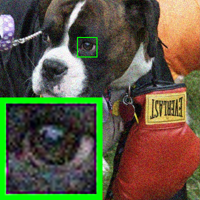
\includegraphics[width=1\textwidth]{images/resize_br_Noisy_dog.png}}
{\footnotesize (a) Noisy Image   }
\end{minipage}
\begin{minipage}[t]{0.25\textwidth}
\centering
\raisebox{-0.15cm}{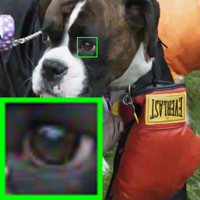
\includegraphics[width=1\textwidth]{images/resize_br_BM3D_dog.png}}
{\footnotesize (b) CBM3D}
\end{minipage}
\begin{minipage}[t]{0.25\textwidth}
\centering
\raisebox{-0.15cm}{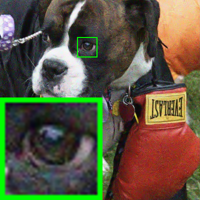
\includegraphics[width=1\textwidth]{images/resize_br_MLP_dog.png}}
{\footnotesize (c) MLP }
\end{minipage}
\begin{minipage}[t]{0.25\textwidth}
\centering
\raisebox{-0.15cm}{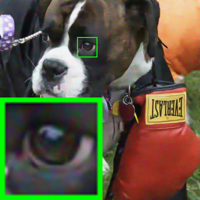
\includegraphics[width=1\textwidth]{images/resize_br_CSF_dog.png}}
{\footnotesize (d) CSF    }
\end{minipage}
}
\subfigure{
\begin{minipage}[t]{0.25\textwidth}
\centering
\raisebox{-0.15cm}{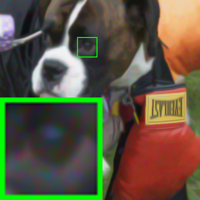
\includegraphics[width=1\textwidth]{images/resize_br_WNNM_dog.png}}
{\footnotesize (e) WNNM    }
\end{minipage}
\begin{minipage}[t]{0.25\textwidth}
\centering
\raisebox{-0.15cm}{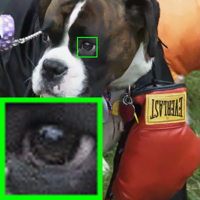
\includegraphics[width=1\textwidth]{images/resize_br_NC_dog.png}}
{\footnotesize (f) Noise Clinic   }
\end{minipage}
\begin{minipage}[t]{0.25\textwidth}
\centering
\raisebox{-0.15cm}{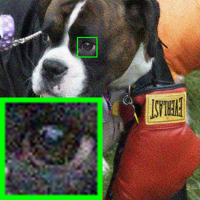
\includegraphics[width=1\textwidth]{images/resize_br_NI_dog.png}}
{\footnotesize (g) Neat Image    }
\end{minipage}
\begin{minipage}[t]{0.25\textwidth}
\centering
\raisebox{-0.15cm}{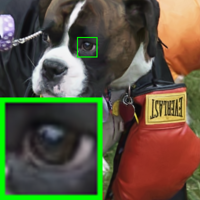
\includegraphics[width=1\textwidth]{images/resize_br_Guided_dog.png}}
{\footnotesize (h) Guided  }
\end{minipage}
}
\caption{Denoised images of the old image "$5dmark3 iso3200 3$" by different methods. The images are better to be zoomed in on screen.}
\label{fig4}
\end{figure*}

%\\
%\hline
%1 &    &    &     &     &    &      &     &     &   & 38.30  &  \textbf{ 40.13 }
%\\
%\hline
%2 &    &    &     &     &    &      &     &     &   & 37.09  &  \textbf{ 36.99 }
%\\
%\hline
%3 &    &    &     &     &    &      &     &     &   & 36.58  &  \textbf{ 36.92 }
%\\
%\hline
%4 &    &    &     &     &    &      &     &     &   & 34.85  &  \textbf{ 35.11 }
%\\
%\hline
%5 &    &    &     &     &    &      &     &     &   &  36.12 &  \textbf{ 36.50 }
%\\
%\hline
%6 &    &    &     &     &    &      &     &     &   & 38.92  &  \textbf{ 38.74 }
%\\
%\hline
%7 &    &    &     &     &    &      &     &     &   & 38.30  &  \textbf{ 38.30 }
%\\
%\hline
%8 &    &    &     &     &    &      &     &     &   &  39.48 &  \textbf{ 40.26 }
%\\
%\hline
%9 &    &    &     &     &    &      &     &     &   & 38.72  &  \textbf{ 38.68 }
%\\
%\hline
%10 &    &    &     &     &    &      &     &     &   & 38.38  &  \textbf{ 38.35 }
%\\
%\hline
%11 &    &    &     &     &    &      &     &     &   & 36.42  &  \textbf{ 36.77 }
%\\
%\hline
%12 &    &    &     &     &    &      &     &     &   & 38.35  &  \textbf{ 38.41 }
%\\
%\hline
%13 &    &    &     &     &    &      &     &     &   & 33.26  &  \textbf{ 33.61 }
%\\
%\hline
%14 &    &    &     &     &    &      &     &     &   &   &  \textbf{ 33.40 }
%\\
%\hline
%15 &    &    &     &     &    &      &     &     &   &   &  \textbf{ 33.47 }

\section{Conclusion and Future Work}

In the future, we will evaluate the proposed method on other conputer vision tasks such as single image super-resolution, photo-sketch synthesis, and cross-domain image recognition. Our proposed method can be improved if we use better training images, fine tune the parameters via cross-validation. We believe that our framework can be useful not just for real image denoising, but for image super-resolution, image cross-style synthesis, and recognition tasks. This will be our line of future work.

{\small
\bibliographystyle{unsrt}
\bibliography{egbib}
}

\end{document}
